\documentclass{article}
\usepackage{graphicx} % Required for inserting images

\title{Test 2}
\author{katkaprudikova}
\date{January 2024}



\begin{document}

\section*{Damped Harmonic Oscillator}

The damped harmonic oscillator is a classic model in physics that describes the motion of a particle under the influence of both a restoring force (harmonic) and a damping force. It is commonly encountered in various physical systems, such as mechanical vibrations and electrical circuits.

\subsection*{Equation of Motion}

The equation of motion for a damped harmonic oscillator is given by the second-order linear differential equation:

\begin{equation}
    m \frac{d^2x}{dt^2} + c \frac{dx}{dt} + kx = 0
\end{equation}

where:
\begin{itemize}
    \item $m$ is the mass of the particle,
    \item $c$ is the damping coefficient,
    \item $k$ is the spring constant,
    \item $x$ is the displacement of the particle as a function of time $t$.
\end{itemize}

This differential equation can also be expressed using the angular frequency $\omega_0$ and the damping ratio $\zeta$ as follows:

\begin{equation}
    \frac{d^2x}{dt^2} + 2\zeta\omega_0\frac{dx}{dt} + \omega_0^2x = 0
\end{equation}

where:
\begin{itemize}
    \item $\omega_0 = \sqrt{\frac{k}{m}}$ is the natural angular frequency,
    \item $\zeta = \frac{c}{2m\omega_0}$ is the damping ratio.
\end{itemize}

\subsection*{Solution}

A possible solution to the damped harmonic oscillator equation is given by the following exponential decay form:

\begin{equation}
    x(t) = e^{-\zeta\omega_0 t}\left(A\cos(\omega_dt) + B\sin(\omega_dt)\right)
\end{equation}

where:
\begin{itemize}
    \item $\omega_d = \omega_0\sqrt{1-\zeta^2}$ is the damped angular frequency,
    \item $A$ and $B$ are constants determined by initial conditions.
\end{itemize}

This solution captures the decay of the oscillations due to the damping effect, and the oscillatory behavior is modulated by the cosine and sine terms.
As shown in Figure \ref{fig:damped_harmonic_oscillator}, the displacement over time follows an exponential decay.

\begin{figure}[h]
    \centering
    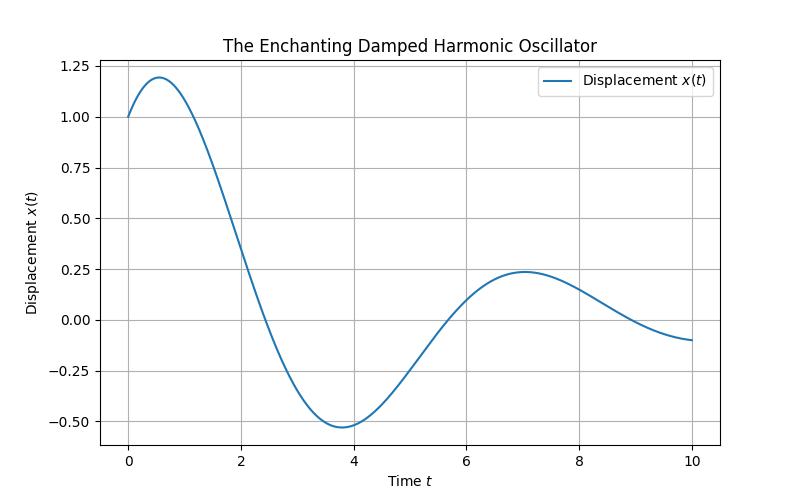
\includegraphics[width=0.8\textwidth]{Figuretest.png} 
    \caption{Damped Harmonic Oscillator: Displacement over Time (in this image m=1; c=0.5; k=1; A=1 and B=1)}
    \label{fig:damped_harmonic_oscillator}
\end{figure}


\end{document}

\maketitle

\section{Introduction}

\end{document}
